% Gemini theme
% https://github.com/anishathalye/gemini

\documentclass[final]{beamer}

% ====================
% Packages
% ====================

\usepackage[T1]{fontenc}
\usepackage{caption}
\usepackage{subcaption}
\usepackage[superscript,biblabel]{cite}
\usepackage{lmodern}
\usepackage[scale=1.15,size=a0,orientation=portrait]{beamerposter}
%\usepackage[size=custom,width=90,height=130,scale=1.25]{beamerposter}
\usetheme{gemini}
\usecolortheme{labsix}
\usepackage{graphicx}
\usepackage{svg}
\svgsetup{inkscapeexe=/Applications/Inkscape.app/Contents/MacOS/inkscape}
\DeclareGraphicsRule{.ai}{pdf}{.ai}{}
\usepackage{booktabs}
\usepackage{tikz}
\usetikzlibrary{fit,backgrounds}
\usepackage{pgfplots}
\usepgfplotslibrary{fillbetween}


% ====================
% Lengths
% ====================

% If you have N columns, choose \sepwidth and \colwidth such that
% (N+1)*\sepwidth + N*\colwidth = \paperwidth
\newlength{\sepwidth}
\newlength{\colwidth}
\setlength{\sepwidth}{0.025\paperwidth}
\setlength{\colwidth}{0.3\paperwidth}

\newcommand{\separatorcolumn}{\begin{column}{\sepwidth}\end{column}}

% ====================
% Title
% ====================

\title{Mesoscopic thermodynamics of single-particle enzymatic reactions}

% REMOVED \inst{1}
\author{Filipe P. de Farias\inst{1} \and Francesco Corona\inst{2}  \and Michela Mulas\inst{1}}

\institute[UFC]{\inst{1}Post-graduate Programme in Teleinformatics Engineering, Federal University of Ceará, Brazil\\ \inst{2}School of Chemical Engineering, Aalto University, Finland}

% ====================
% Footer (optional)
% ====================
 %% REMOVED {  %\href{https://www.example.com}{https://www.example.com} 
  %\href{mailto:alyssa.p.hacker@example.com}{alyssa.p.hacker@example.com} }
\footercontent{
  \hfill
  Challenges in the Physics of Active and Biological Matter 2023
  \hfill
}
% (can be left out to remove footer)

% ====================
% Logo (optional)
% ====================

% use this to include logos on the left and/or right side of the header:
\logoright{\includegraphics[height=10cm,
%page=2,trim={17cm 21cm 3cm 5cm},clip
]{"graphics/brasao2_vertical_monocromatico"}}
\logoleft{\includegraphics[height=10cm,trim={50 50 50 50},clip]{"graphics/logo-31148-1"}}

% ====================
% Body
% ====================

\begin{document}

\setlength{\abovedisplayskip}{40pt}
\setlength{\belowdisplayskip}{40pt}

\begin{frame}[t]
\begin{columns}[t]
\separatorcolumn

\begin{column}{\colwidth}

%\begin{block}{Introduction}
%The energy transfer of systems at mesoscopic scale with stochastic dynamics which are open and out-of-equilibrium are the subject of study Stochastic Thermodynamics\cite{peliti2021stochastic,Falasco:2023aa}. 
%%
%\begin{itemize}
%\item Systems at equilibrium have {\bf reversible trajectory}, i.e. a transition of the system from the state $x \rightarrow x^\prime$ at a rate $k_{xx^\prime}$, its reversed transition $x^\prime \rightarrow x$ has the rate $k_{x^\prime x}=k_{xx^\prime}$.
%
%\item At {\bf non-equilibrium} a system is kept stationary by dissipating energy (local detailed balance) proportional to $\ln (k_{xx^\prime} / k_{x^\prime x})$\cite{10.21468/SciPostPhysLectNotes.32}.
%\end{itemize}
%{\bf Stochastic thermodynamics} (ST) deals with the interaction of mesoscopic, nonequilibrium physical systems with heat reservoirs in equilibrium.\cite{peliti2021stochastic} Such interactions are assumed to be the source of the randomness in the dynamics of the system, assigning to it a probability $p_x(t)$ of being in the state $x$ at time $t$.
%\begin{itemize}
%\item We will use the Michaelis-Menten kinetics as case of study for the ST.
%\end{itemize}
%\end{block}

\begin{block}{Michaelis-Menten theory}
The transitions in the Michaelis-Menten case represent the changes in the configuration of the single enzyme ($E$) to complexed with substrate ($ES$) and back.
\begin{itemize}
\item The reaction network that models the kinetics is:
\begin{equation}
E + S \underset{k_{-1}}{\stackrel{k_1}{\rightleftharpoons}} ES \underset{k_{-2}}{\stackrel{k_2}{\rightleftharpoons}} E + P
\end{equation}
%
where $P$ is the product of the complete process.
%
\item The transitions occur due to the random interactions of the enzyme with the solution, the later acting as a reservoir in equilibrium with defined temperature T\cite{Seifert:2010aa}.

\begin{figure}
\centering
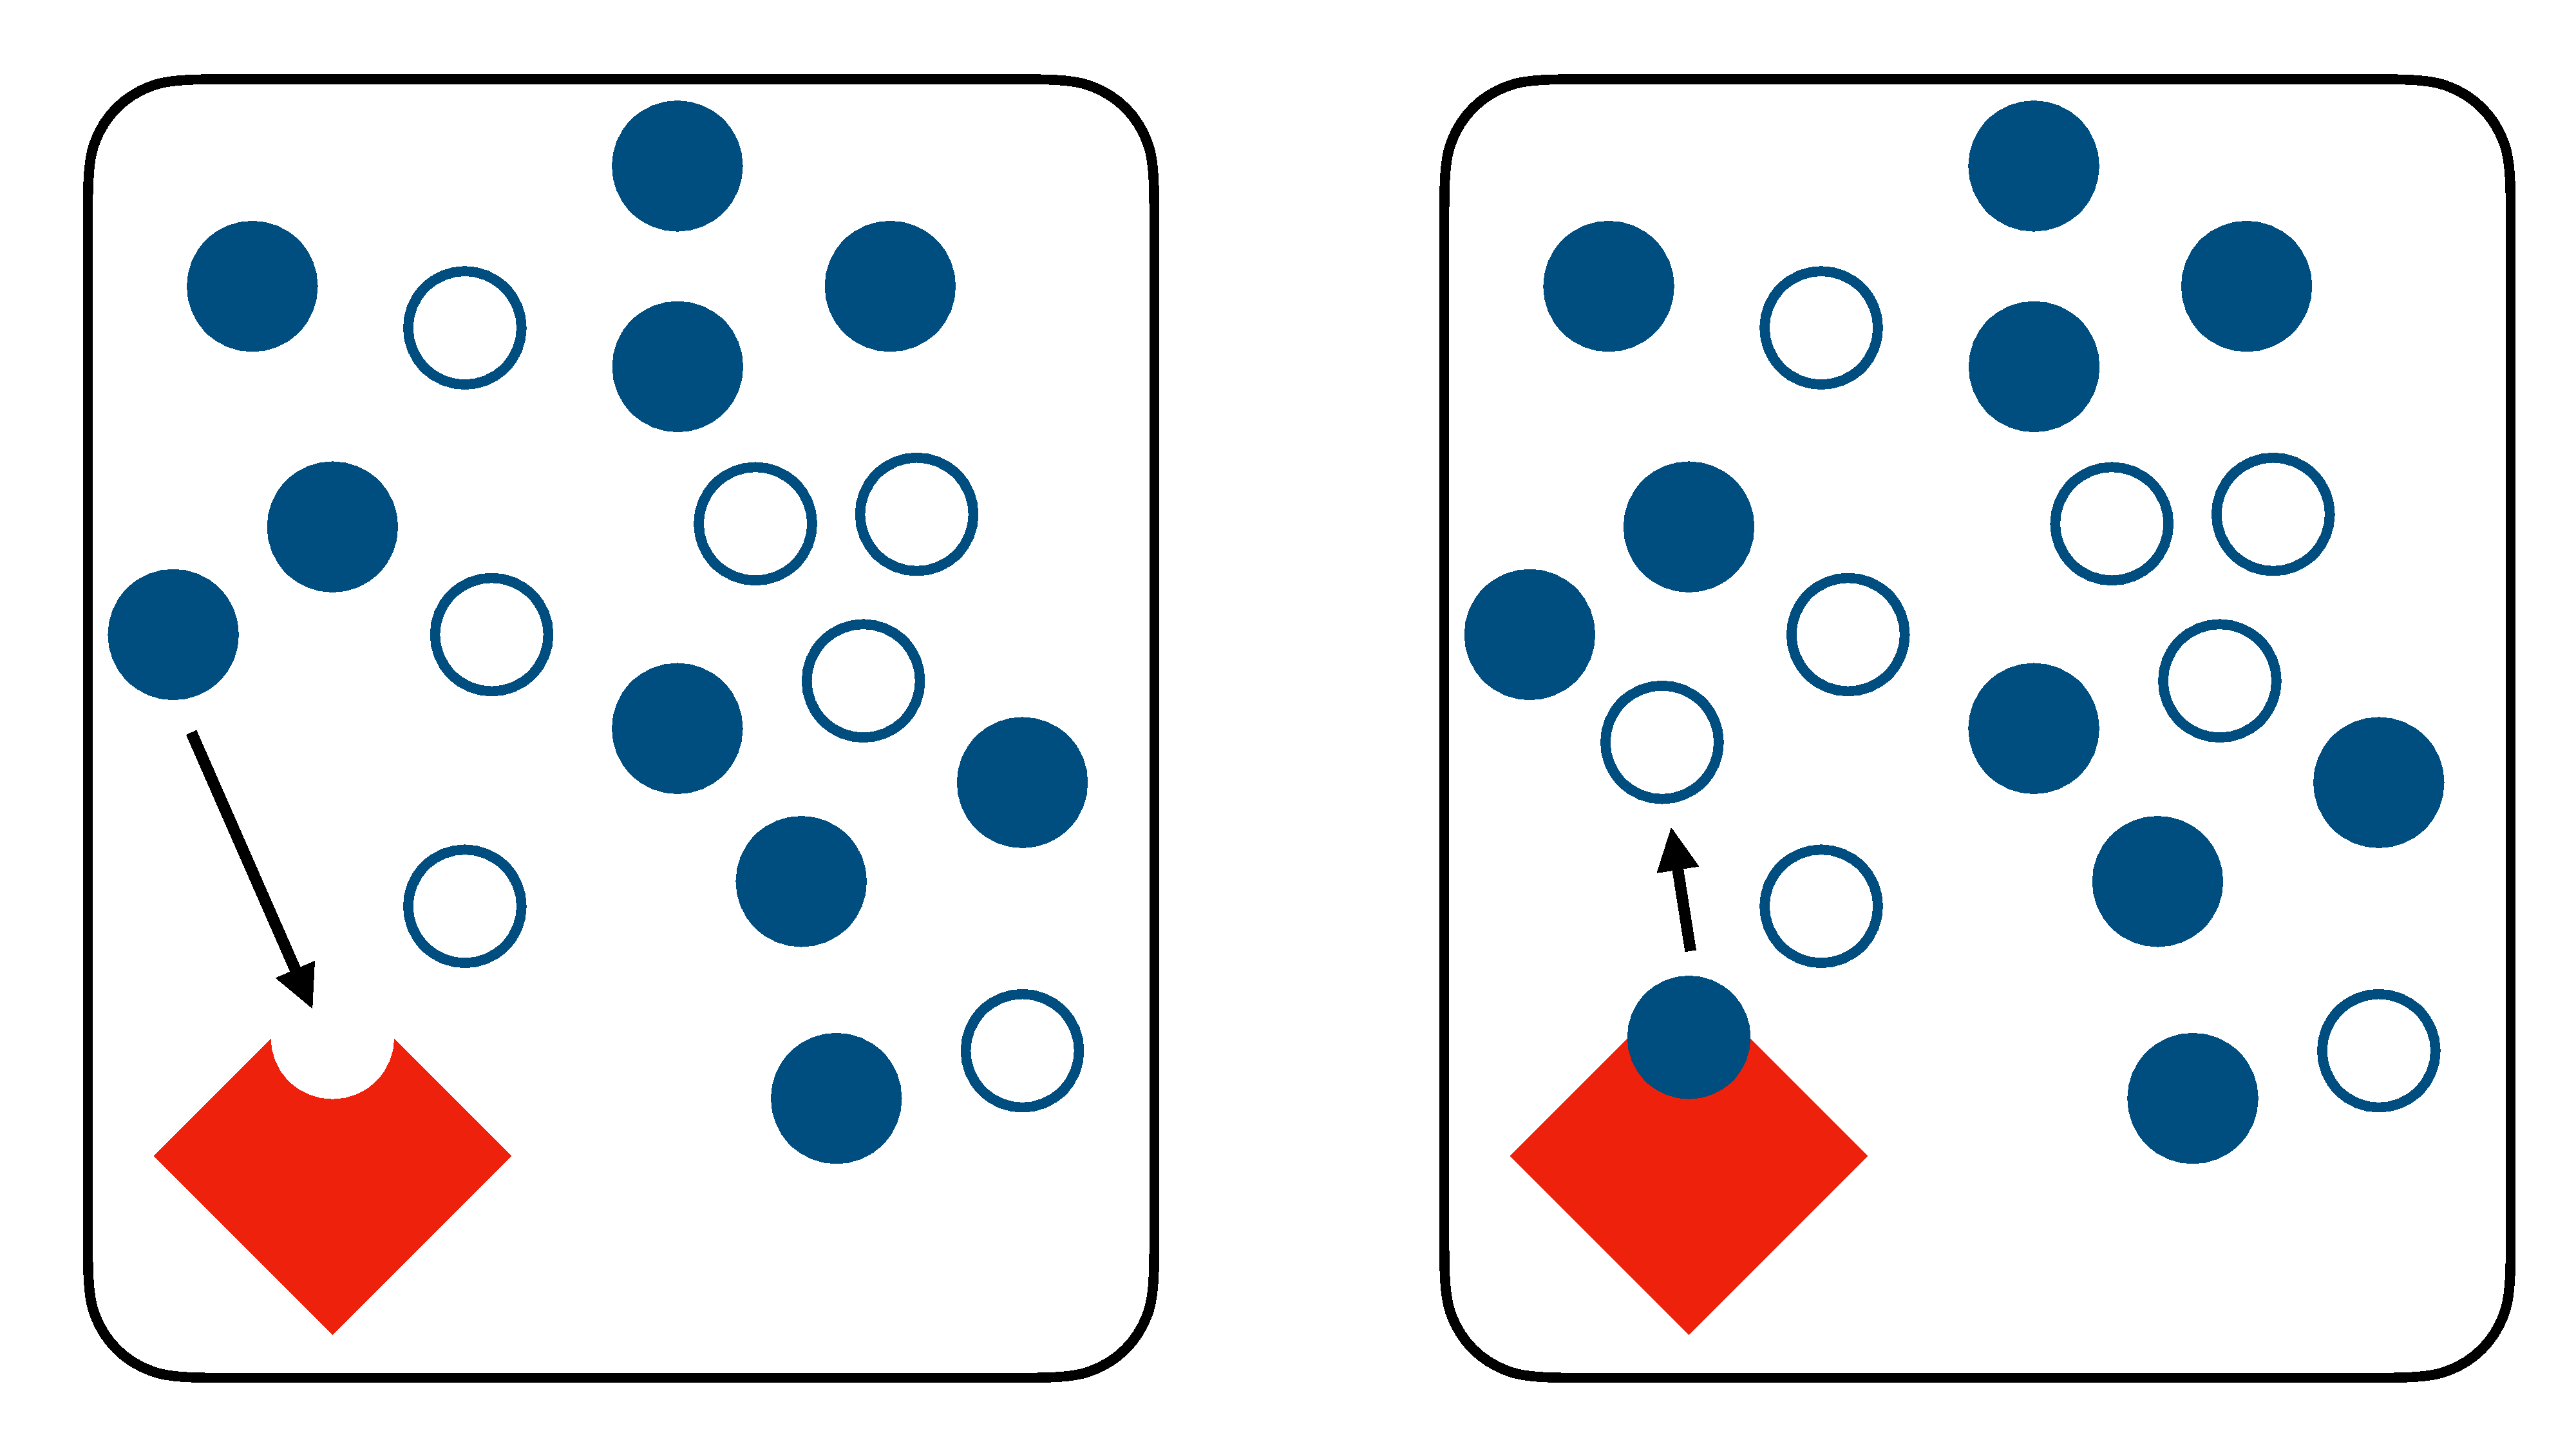
\includegraphics[width=.8\textwidth]{graphics/MichaelisMenten.pdf}
\caption{Figure adapted from Seifert (2010)\cite{Seifert:2010aa}, where the solution is composed by substrate (filled circle), product (empty circle) and single enzyme (red). The single enzyme is randomly interacting with the solution changing its state.}
\vskip-40pt
\end{figure}
%
%\item The substrate $S$ and the product $P$ are {\bf chemostated}.
%\begin{figure}
%\begin{subfigure}[b]{0.45\textwidth}
%\centering
%\includesvg{graphics/2-state-graph.svg}
%\caption{}
%\label{fig 2-state-system}
%\end{subfigure}
%\begin{subfigure}[b]{0.45\textwidth}
%\centering
%\includesvg[scale=1.1]{graphics/ST-MM-prob.svg}
%\caption{}
%\label{fig 2-prob-evol}
%\end{subfigure}
%\caption{In (a) a single trajectory of the system using the Gillespie algorithm. In (b) the time evolution of the probability of each state of the system.}
%\end{figure}
%\item The observation of a single realization of this system is given in Figure \ref{fig 2-state-graph}. The system fluctuates between the two states until reaches a stationary configuration.
\item The system performs a Markovian jump process with the states having probability\cite{GILLESPIE1976403} given by the solution of the following {\bf Master equation}\cite{van2007stochastic}
%
\begin{equation}
\frac{dp_x(t)}{dt} = \sum_x W_{x^\prime x} p_x(t) -  W_{x x^\prime}p_{x^\prime}(t) \label{eq CME}
\end{equation}
\item The $W_{x x^\prime }$ is the {\bf probability transition rate} from the state $x^\prime$ to $x$, it forms a {\bf stochastic matrix} $W$ dependent on the kinetics of the chemical reactions\cite{Munsky_2006}:
\begin{equation}
W_{x^\prime x} =
-\sum_\nu a_\nu({x}_{\nu}) \delta(x - x^\prime) + a_\nu({x}_{\nu}) \delta(x - x^\prime - s_\nu),
\end{equation}
\vskip-20pt
where were defined:\\
%\begin{itemize}
%\item 
- The {\bf propensity function} $a_\nu({x}) = \prod_i k_\nu \frac{{x}_{i}!}{({x}_{i} - s_{i,\nu})!}$ for each $\nu$-th reaction,  with the vector of states $x = [x_1,...,x_i,...]$ and state changes $s = [s_1,...,s_i,...]$;\\
%\item 
- ${x}_{i,\nu} $ as the number of molecules in the system of the i-th reactant in the $\nu$-th reaction;\\
%\item 
- $s_{i,\nu} $ as the number of molecules of the i-th reactant participating in the $\nu$-th reaction.
%
%\end{itemize}
%\item Integrating or sampling \eqref{eq CME} allow us to obtain the probabilities $p_x(t)$.
%\item 
\end{itemize}
\end{block}


\begin{alertblock}{References}

%\nocite{*}
\footnotesize{\bibliographystyle{plain}\bibliography{poster-Phys-ActBio-Matter-2023}}

\end{alertblock}
%
%\begin{figure}
%\label{fig 1}
%\begin{subfigure}[b]{0.45\textwidth}
%\includesvg{graphics/ST-1.svg}
%\caption{}
%\label{fig 2-state-system}
%\end{subfigure}
%\hfill
%\begin{subfigure}[b]{0.45\textwidth}
%\end{subfigure}
%\caption{In (\subref{fig 2-state-system}) the representation of the MM[Massimiliano REF?] and in (\subref{fig 2-state-graph}) a single realization of the system.}
%\end{figure}
%
%
%The system is kept in contact with a heat bath with temperature $T$.
%\begin{itemize}
%\item The changes in state of the system are due to energy exchanges with the bath.
%\end{itemize}
%
%\begin{block}{Master Equation}
%The probability $p_x(t)$ of the system being in $x \in \{E,ES\}$ and how it changes with time, is given by a {\bf master equation}\cite{van2007stochastic}. It reads:
%%
%\begin{equation}
%\frac{dp_x(t)}{dt} = \sum_x W_{x^\prime x} p_x(t) -  W_{x x^\prime}p_{x^\prime}(t) \label{eq CME}
%\end{equation}
%\begin{itemize}
%\item The $W_{x^\prime x}$ is the {\bf probability transition rate} from the state $x^\prime$ to $x$, it forms a {\bf stochastic matrix} $W$ dependent on the kinetics of the chemical reactions\cite{GILLESPIE1976403}:
%\begin{equation}
%W_{x^\prime x} = \sum_\nu \prod_i k_\nu \frac{x_{i,\nu}!}{(x_{i,\nu} - s_{i,\nu})!}
%\end{equation}
%$x_{i,\nu} = $ \# of molecules in the system of the i-th reactant in the $\nu$-th reaction.\\
%$s_{i,\nu} = $ \# of molecules of the i-th reactant participating in the $\nu$-th reaction.
%%\item Integrating or sampling \eqref{eq CME} allow us to obtain the probabilities $p_x(t)$.
%%\item 
%\end{itemize}
%\end{block}

\end{column}

\separatorcolumn

\begin{column}{\colwidth}

%\begin{block}{\vphantom{a}}
%\end{block}

\begin{block}{Stochastic Thermodynamics (ST)}
\vskip10pt
%\begin{figure}
%\label{fig 1}
%\begin{subfigure}[b]{0.45\textwidth}
%\centering
%\includesvg{graphics/ST-1.svg}
%\caption{}
%\label{fig 2-state-system}
%\end{subfigure}
%\begin{subfigure}[b]{0.45\textwidth}
%\centering
%\includesvg[scale=1.1]{graphics/ST-MM-prob.svg}
%\caption{}
%\label{fig 2-prob-evol}
%\end{subfigure}
%\caption{In (\subref{fig 2-state-system}) the representation of MM\cite{esposito2023} and in (\subref{fig 2-prob-evol}) the evolution of the probability for each state.}
%\end{figure}
%The classical thermodynamics is defined assumed an {\bf equilibrium} situation of the system.
%
The energy transfer of systems at mesoscopic scale with stochastic dynamics which are open and out-of-equilibrium is the subject of study Stochastic Thermodynamics\cite{peliti2021stochastic,Falasco:2023aa}. 
%
\begin{itemize}
\item Systems at equilibrium have {\bf reversible trajectory}, i.e. a transition of the system from the state $x \rightarrow x^\prime$ at has the rate $W_{xx^\prime}$ and its reversed transition $x^\prime \rightarrow x$ has the rate $W_{x^\prime x}=W_{xx^\prime}$.

\item At {\bf non-equilibrium} a system is kept stationary by dissipating energy (local detailed balance, LDB) proportional to $\ln (W_{xx^\prime} / W_{x^\prime x})$ in each transition\cite{10.21468/SciPostPhysLectNotes.32}.
\end{itemize}
%The local detailed balance (LDB) is the link between ST and classical thermodynamics\cite{Falasco:2023aa}:
\begin{itemize}
\item The transition $x \rightarrow x^\prime$ must expel/absorb an amount of entropy equals to
%
\begin{equation}
s(t) = k_B T \ln \frac{W_{xx^\prime}}{W_{x^\prime x}}
\end{equation}
%
\item Solving \eqref{eq CME}, one obtains the probabilities to compute the {\bf average rate entropy flux} which is expelled/absorbed by the reservoir\cite{peliti2021stochastic}:
%
\begin{equation}
\dot{S}^{res} = k_B T \frac{1}{2} \sum_{x \neq x^\prime} \left[ W_{x^\prime x} p_x(t) -  W_{x x^\prime}p_{x^\prime}(t) \right] \ln \frac{W_{x^\prime x}}{W_{xx^\prime}}
\end{equation}
%
\item From the average, one obtains the relations for the {\bf average entropy production rate} and {\bf entropy balance rate}\cite{Schnakenberg:1976aa}, respectively:
%
\begin{subequations}
\begin{equation}
\dot{S}^{tot}  = k_B T\frac{1}{2} \sum_{x \neq x^\prime} \left[ W_{x^\prime x} p_x(t) -  W_{x x^\prime}p_{x^\prime}(t) \right] \ln \frac{W_{x^\prime x} p_x(t)}{W_{xx^\prime}p_{x^\prime}(t)};
\end{equation}
\begin{equation}
 \dot{S}^{sys} = k_B T \frac{1}{2} \sum_{x \neq x^\prime} \left[ W_{x^\prime x} p_x(t) -  W_{x x^\prime}p_{x^\prime}(t) \right] \ln \frac{p_x(t)}{p_{x^\prime}(t)}.
\end{equation}
\end{subequations}

\end{itemize}




%\item In the ST, the equilibrium is held by the bath, the system is allowed to be in {\bf nonequilibrium}.
%%\item When the system reaches the equilibrium, it is also in equilibrium with the bath (Zero-th law).
%\item In such case, ST gives that the system has nonnegative {\bf average entropy production rate} $\dot{S}^{sys}$:
%%
%\begin{equation}
%\dot{S}^{sys} = k_B T \frac{1}{2} \sum_{x \neq x^\prime} \left[ W_{x^\prime x} p_x(t) -  W_{x x^\prime}p_{x^\prime} \right] \ln \frac{p_x(t)}{p_{x^\prime}(t)}.
%\end{equation}
%%
%This expression can be separated in two parts:
%\begin{subequations}
%\begin{equation}
%\dot{S}^{tot}  = k_B T\frac{1}{2} \sum_{x \neq x^\prime} \left[ W_{x^\prime x} p_x(t) -  W_{x x^\prime}p_{x^\prime} \right] \ln \frac{W_{x^\prime x} p_x(t)}{W_{xx^\prime}p_{x^\prime}(t)}
%\end{equation}
%\begin{equation}
%\dot{S}^{bath}  = k_B T \frac{1}{2} \sum_{x \neq x^\prime} \left[ W_{x^\prime x} p_x(t) -  W_{x x^\prime}p_{x^\prime}(t) \right] \ln \frac{W_{x^\prime x}}{W_{xx^\prime}}
%\end{equation}
%\end{subequations}
%The term $\dot{S}^{bath}$ is the average heat absorbed by the bath when the system jumps between the states, while $\dot{S}^{tot}$ is the total entropy change (or balance) of the universe (system plus bath).
\end{block}
\begin{block}{}
The probability of the state when the system is in equilibrium $p_x^{eq}$ gives the {\bf generalized free energy rate}\cite{Qian_2021}:

\begin{equation}
\label{eq noneq free en}
\dot{F}(t) - \dot{F}^{eq}(t)= \sum_{x \neq x^\prime} \left[ W_{x^\prime x} p_x(t) -  W_{x x^\prime}p_{x^\prime}(t) \right] \ln \frac{p_x(t)}{p_{x^\prime}^{eq}},
\end{equation}
%
where $\dot{F}^{eq}$ is the equilibrium free energy rate.
\begin{itemize}
\item The nonequilibrium free energy rate in \eqref{eq noneq free en} is defined as the information $I$ needed to specify the nonequilibrium state\cite{Esposito_2011}, thus
%
\begin{equation}
{F}(t) - {F}^{eq}(t) = k_B TI(t) \equiv TD_{KL}(p_x(t) || p_x^{eq}(t)) \geq 0
\end{equation}
%
where $D_{KL}$ is the Kullback-Leibler divergence measuring the ``difference'' between the nonequilibrium and the equilibrium probability distributions.
%The difference between  the rate of work which is done when we manipulate the system $\dot{w}$ and the one available to be extracted $\dot{F}^{eq}$ is
%\begin{equation}
%\dot{w} - \dot{F}^{eq}= \frac{1}{2} \sum_{x \neq x^\prime} \left[ W_{x^\prime x} p_x(t) - W_{x x^\prime}p_{x^\prime} \right] \ln \frac{W_{x^\prime x} p_x^{eq}}{W_{xx^\prime}p_{x^\prime}^{eq}}.
%\end{equation}
%\item The thermodynamic flux and force are defined as, respectively
%%
%\begin{equation}
%J_{xx^\prime} = W_{x^\prime x} p_x(t) -  W_{x x^\prime}p_{x^\prime}(t) \qquad A_{xx^\prime} =  \ln \frac{W_{x^\prime x} p_x(t)}{W_{xx^\prime}p_{x^\prime}(t)}
%\label{eq therm-flux-force}
%\end{equation}
\end{itemize}
\end{block}

\begin{block}{}
{\bf Fluctuation theorems} set constrains on the distributions of the observables above:
\begin{itemize}
\item The {\bf integral} and the {\bf detailed} fluctuation relation constrain the entropy production\cite{peliti2021stochastic}
\begin{equation}
\langle e^{s(t)/k_BT} \rangle_F = 1, \quad \frac{p(s)}{p(-s)} = e^{s/k_B T}.
\end{equation}
%\item The {\bf detailed fluctuation relation} constrains the entropy production\cite{peliti2021stochastic}
%
\end{itemize}
%
There are other relations as Crooks and Jarzynski relations which deal with the fluctuations in the work applied to the system. They are, respectively:
%
\begin{equation*}
\langle e^{-w/k_B T} \rangle_F = e^{-\Delta F/k_BT}, \quad \frac{p(w;\lambda)}{p(-w;\hat{\lambda})} = e^{(w - \Delta F)/k_B T}.
\end{equation*}
%
But as there is no driving or control protocol $\lambda$ (and its time-reversed $\hat{\lambda}$), the analysis will not be done in this work,
\end{block}

\end{column}

\separatorcolumn

\begin{column}{\colwidth}

\begin{block}{Results}
The system was simulated using the parameters  $k_{1} = 0.5$, $k_{-1} = 0.005$, $k_{2} = 0.1$ and $k_{-2} = 0.0$.
\begin{figure}
%\vskip-30pt 
\begin{center}
%\includesvg[scale=1.25]{graphics/ST-MM-2.svg}
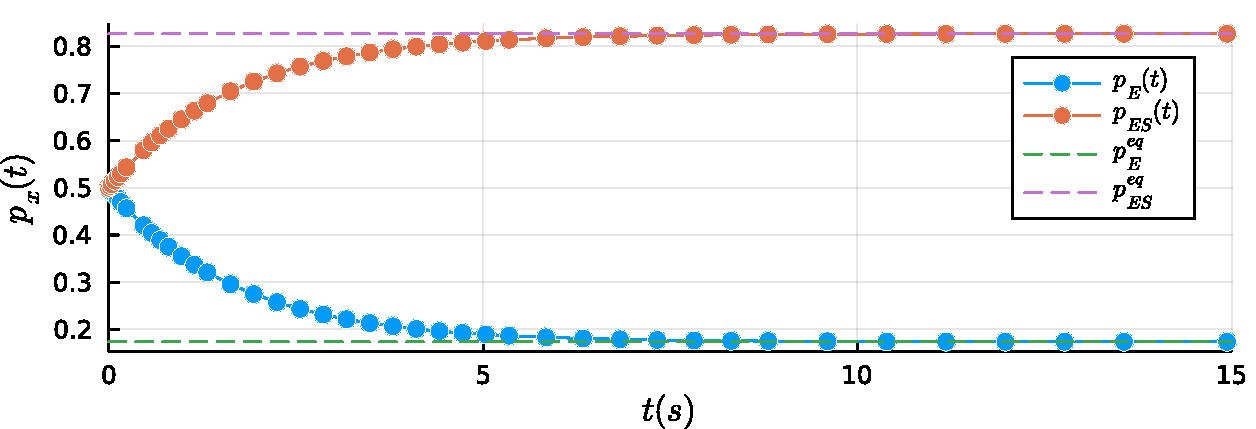
\includegraphics[scale=1.2]{graphics/f1.pdf}
\end{center}
\label{fig 2-state-system}
\caption{The time evolution of the system compared to its equilibrium probability values.}
\end{figure}

\begin{figure}
%\vskip-30pt 
\begin{center}
%\includesvg[scale=1.25]{graphics/ST-MM-2.svg}
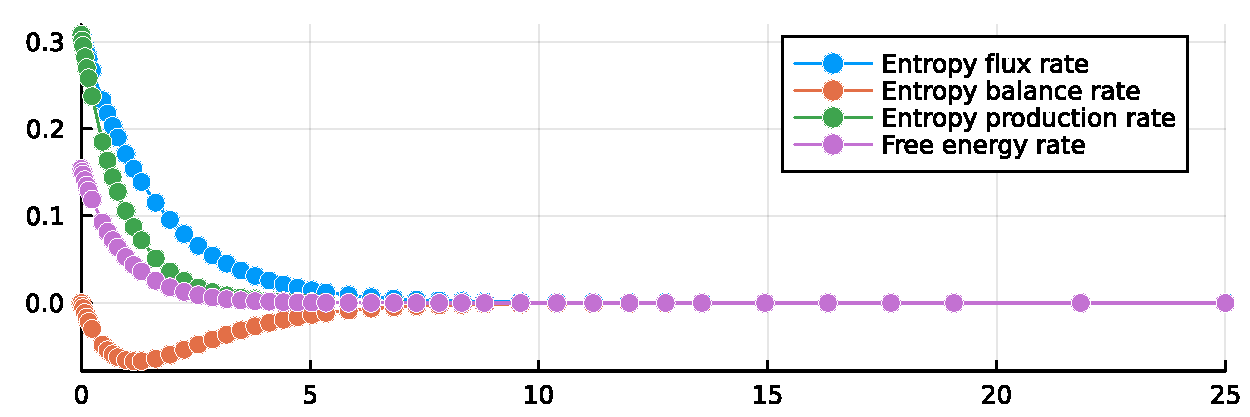
\includegraphics[scale=1.2]{graphics/f2.pdf}
\end{center}
\label{fig 2-state-system}
\caption{Average entropy flux, balance, production ans free energy rates evaluated according to ST.}
\end{figure}

Below are shown 5 different trajectories of the system and the thermodynamic observables in each one.

\begin{figure}
%\vskip-30pt 
\begin{center}
%\includesvg[scale=1.25]{graphics/ST-MM-2.svg}
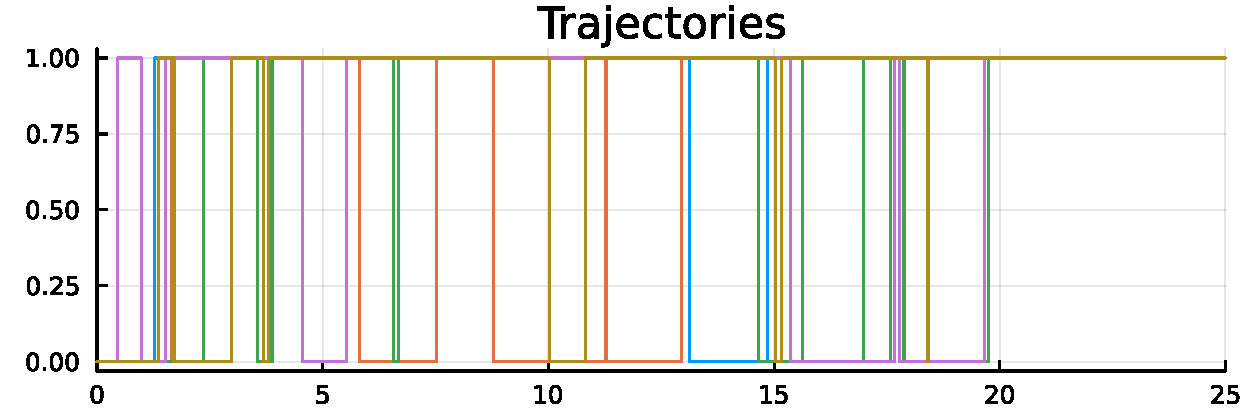
\includegraphics[scale=1.2]{graphics/f6.pdf}
\end{center}
\label{fig 2-state-system}
\caption{Simulation of the Markov jump process for the Michaelis-Menten. Each color is a different trajectory of the system. The enzyme jumps from the state $E$ (0.00 in $y$-axis) to $ES$ (1.00 in $y$-axis).}
\end{figure}

\begin{figure}
%\vskip-30pt 
\begin{center}
%\includesvg[scale=1.25]{graphics/ST-MM-2.svg}
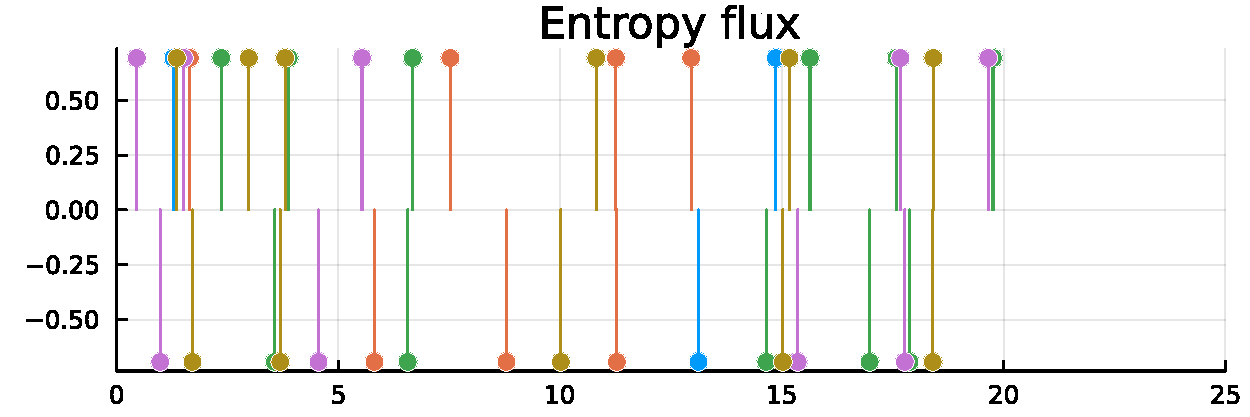
\includegraphics[scale=1.2]{graphics/f3.pdf}
\end{center}
\label{fig 2-state-system}
\caption{Stochastic entropy flux per $k_B T$ released in each transition in time. Each color is a different trajectory of the system.}
\end{figure}

\begin{figure}
%\vskip-30pt 
\begin{center}
%\includesvg[scale=1.25]{graphics/ST-MM-2.svg}
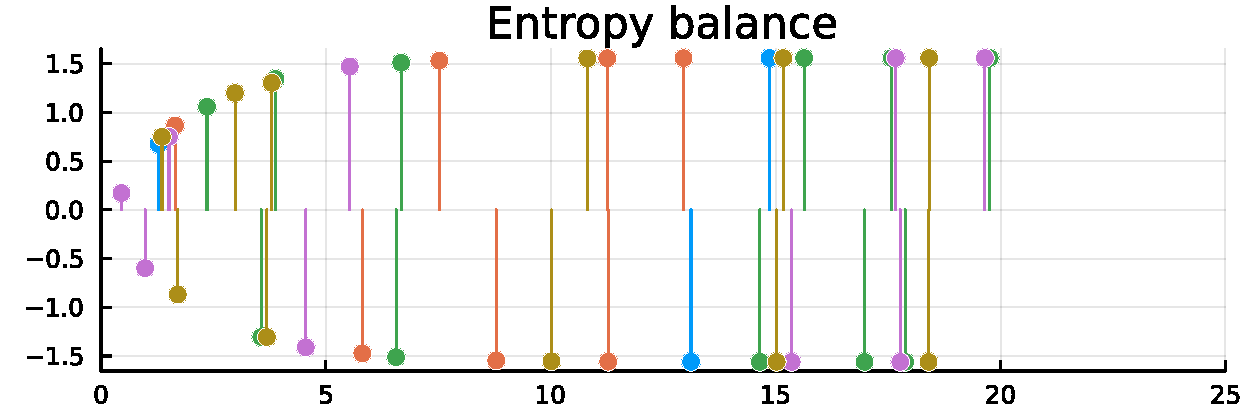
\includegraphics[scale=1.2]{graphics/f4.pdf}
\end{center}
\label{fig 2-state-system}
\caption{Stochastic entropy balance per $k_B T$ released in each transition in time. Each color is a different trajectory of the system.}
\end{figure}

\begin{figure}
%\vskip-30pt 
\begin{center}
%\includesvg[scale=1.25]{graphics/ST-MM-2.svg}
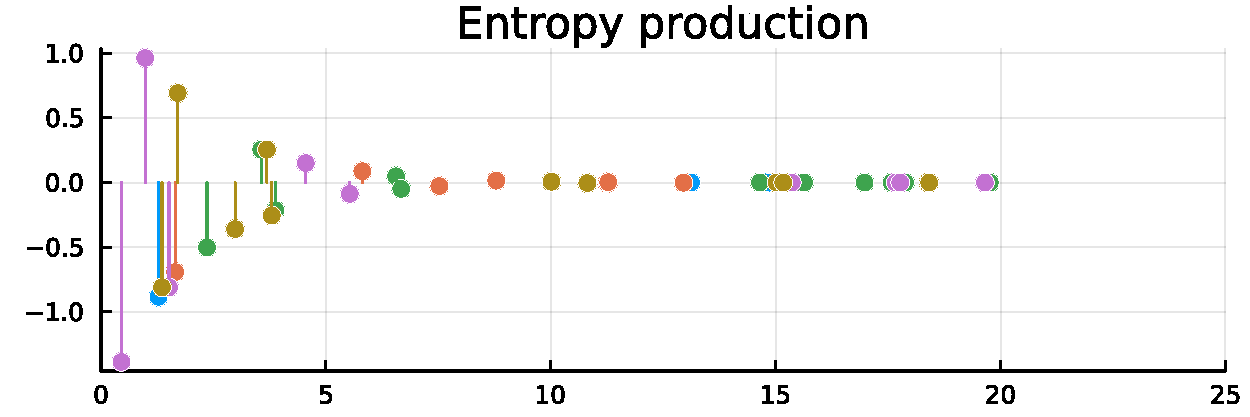
\includegraphics[scale=1.2]{graphics/f5.pdf}
\end{center}
\label{fig 2-state-system}
\caption{Stochastic entropy production per $k_B T$ released in each transition in time. Each color is a different trajectory of the system..}
\end{figure}

%The system reaches the steady-state, which for the case of study happens to be also the equilibrium in about 10 seconds:
%
%\begin{itemize}
%\item Both\cite{Qian_2021} the thermodynamic force and flux vanish in the steady-state, which is also an equilibrium.
%
%
%
%
%%\item It can be verified that the system obeys {\bf detailed balance}, which connects the math and the physics by recovering the Boltzmann distribution.
%
%\item It can be noticed also that all the free energy is used to produce entropy.
%
%\item This could be different if one realize work on the system, and it's subject of further research.
%\end{itemize}
\end{block}


\end{column}

\separatorcolumn
\end{columns}
 \end{frame}
\end{document}
